\documentclass[14pt, a4paper]{extarticle}

\usepackage[utf8]{inputenc}
\usepackage[T1]{fontenc}
\usepackage{amsmath}
\usepackage{amssymb}
\usepackage{graphicx}
\usepackage[left=2.00cm, right=2.00cm, top=2.00cm, bottom=2.00cm]{geometry}
\usepackage[russian]{babel}

\usepackage{setspace}
\usepackage{fancyhdr}

\graphicspath{{img/}}

\RequirePackage{caption}
\captionsetup[figure]{justification=centering,name=Рисунок,labelsep=endash}

\usepackage{indentfirst}

\usepackage{float}

\begin{document}
	\onehalfspacing
	\begin{titlepage}
	\begin{center}
		\begin{small}
			\textbf{Министерство науки и высшего образования Российской Федерации}

			ФЕДЕРАЛЬНОЕ ГОСУДАРСТВЕННОЕ АВТОНОМНОЕ ОБРАЗОВАТЕЛЬНОЕ УЧРЕЖДЕНИЕ ВЫСШЕГО ОБРАЗОВАНИЯ
			
			\textbf{<<НАЦИОНАЛЬНЫЙ ИССЛЕДОВАТЕЛЬСКИЙ УНИВЕРСИТЕТ ИТМО>>}
		\end{small}
		
		\vspace{8em}
		
		Отчет по лабораторной работе №4
		
		СИНТЕЗ ОПТИМАЛЬНОГО УПРАВЛЕНИЯ. ПРИНЦИП МАКСИМУМА
		
		По дисциплине <<Оптимальное управление>>
	\end{center}
	
	\vspace{8em}
	
	\begin{flushright}
		Выполнил:\\
		студент группы R42331c\\
		Манахов~С.П.
		
		\vspace{1em}
		
		Преподаватель:\\
		Парамонов~А.В.
	\end{flushright}

	\vfill
	
	\begin{center}
		\small
		Санкт-Петербург\\
		2022 г.\\
	\end{center}
\end{titlepage}
	\setcounter{page}{2}
	
	\section*{Задание}
	
	\begin{enumerate}
		\item Рассчитать коэффициенты оптимального регулятора для линейного объекта:
		$$\dot{x}=Ax+bu, x(0)$$
		Структура регулятора $u=-Kx$. Расчет произвести на основе уравнения Риккати:
		$$A^TP+PA+Q-Pbr^{-1}b^TP=0$$
		$$K=r^{-1}b^TP$$
		и критерия качества вида:
		$$J=\int\limits_{0}^{\infty}x^T(\tau)Qx(\tau)+ru^2(\tau)d\tau$$
		\item Произвести моделирование замкнутой системы при начальных условиях $x(0)=[1,0]^T$. Построить графики моделирования $x_1,x_2,u$ и $J$. Рассчитать установившееся значение $J$;
		\item Незначительно отклонить расчетные значения $K$ так, чтобы система сохранила устойчивость, и повторить п.~2 при том же времени моделирования. Сравнить с результатами п.~2 и сделать выводы;
		\item Провести моделирование для трех разных значений параметра $r$ и трех разных матриц $Q$ при условиях, что $r>0$, $Q=kQ^*$, $k$ -- положительный коэффициент, матрица $Q^*$ равна исходной матрице $Q$ в соответствии с вариантом задания. По результатам экспериментов построить графики моделирования $x_1,x_2,u$ и $J$.
	\end{enumerate}
	\begin{table}[H]
		\centering
		\begin{tabular}{|c|c|c|c|c|}
			\hline
			Вариант & Матрица $A$ & Матрица $b$ & Матрица $Q$ & Параметр $r$ \\\hline
			9 & 
			$\left[
			\begin{matrix}
				0 & 1 \\
				0 & 0 
			\end{matrix}
			\right]$
			& 
			$\left[
			\begin{matrix}
				0 \\ 5
			\end{matrix}
			\right]$
			& 
			$\left[
			\begin{matrix}
				2 & 0 \\
				0 & 3 
			\end{matrix}
			\right]$
			& 4 \\\hline
		\end{tabular}
	\end{table}
	
	\newpage
	
	\section*{Описание работы}
	
	Полученная при помощи пакета \textit{MATLAB~Simulink} система представлена на рисунках \ref{fig:system}--\ref{fig:MATLAB-Function}.
	
	\begin{figure}[H]
		\centering
		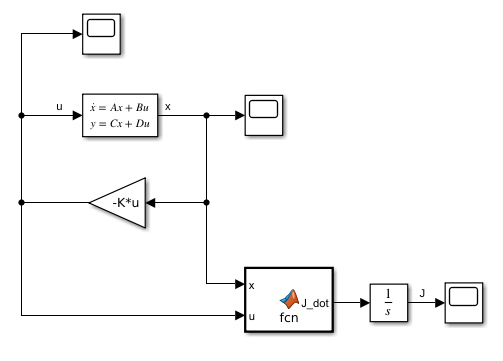
\includegraphics[width=0.6\textwidth]{system}
		\caption{Замкнутая система}
		\label{fig:system}
	\end{figure}

	\begin{figure}[H]
		\centering
		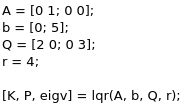
\includegraphics{properties}
		\caption{Параметры системы}
		\label{fig:properties}
	\end{figure}

	\begin{figure}[H]
		\centering
		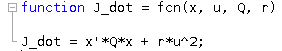
\includegraphics{MATLAB-Function}
		\caption{Блок MATLAB-Function}
		\label{fig:MATLAB-Function}
	\end{figure}

	Произведем моделирование системы при начальных условиях $x(0)=[1,0]^T$. Полученные графики представлены на рисунках \ref{fig:x-2}--\ref{fig:J-2}.

	\begin{figure}[H]
		\centering
		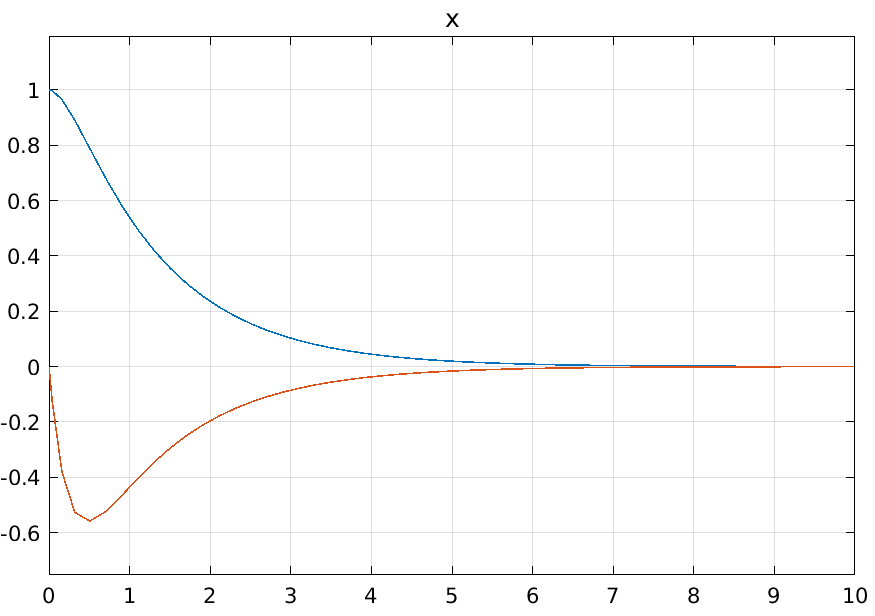
\includegraphics[width=0.59\textwidth]{x-2}
		\caption{Вектор состояния системы $x$ при $x(0)=[1,0]^T$}
		\label{fig:x-2}
	\end{figure}

	\begin{figure}[H]
		\centering
		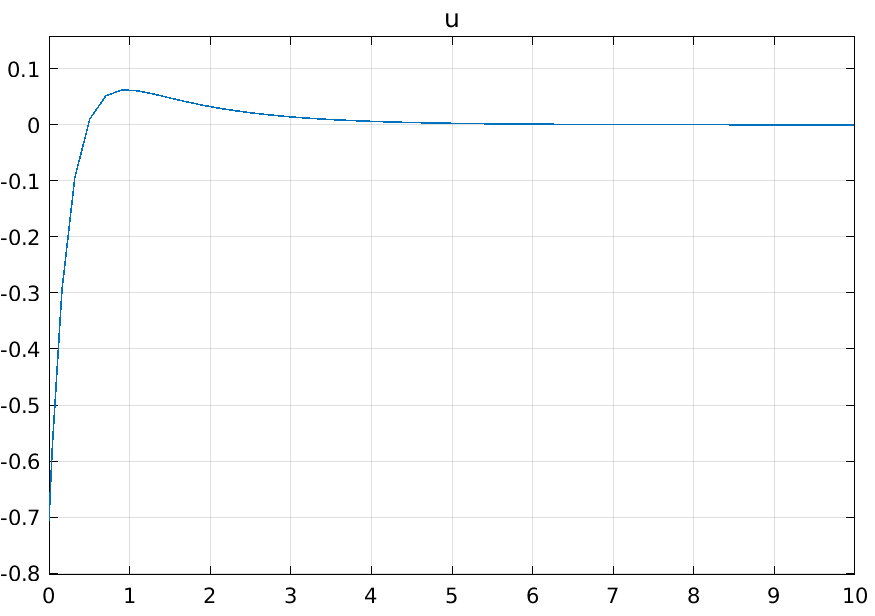
\includegraphics[width=0.59\textwidth]{u-2}
		\caption{Управляющий сигнал $u$ при $x(0)=[1,0]^T$}
		\label{fig:u-2}
	\end{figure}

	\begin{figure}[H]
		\centering
		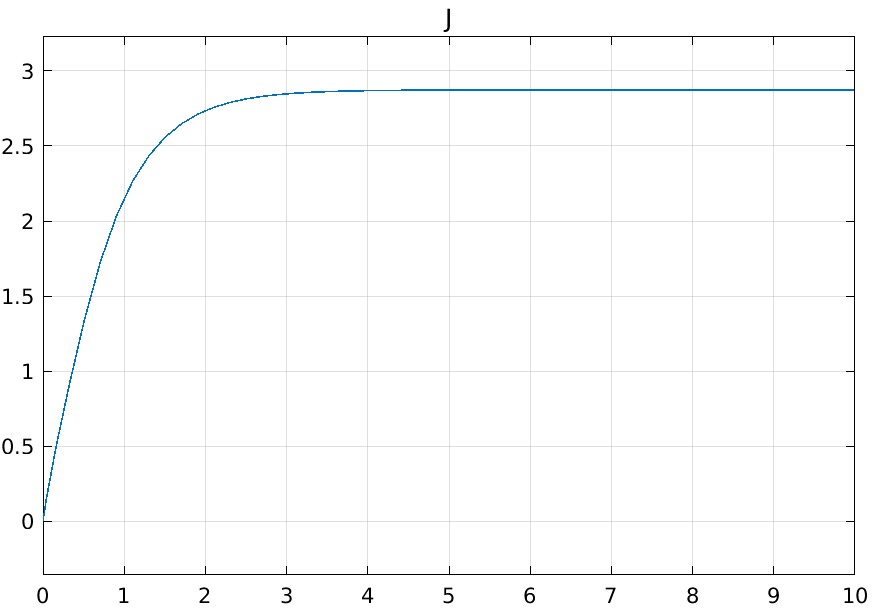
\includegraphics[width=0.59\textwidth]{J-2}
		\caption{Критерий качества $J$ при $x(0)=[1,0]^T$}
		\label{fig:J-2}
	\end{figure}

	Установившееся значение критерия качества $J=2,8739$.
	
	Теперь незначительно отклоним расчетное значение $K$ в положительную сторону $K+1$. Полученные графики представлены на рисунках \ref{fig:x-3-plus}--\ref{fig:J-3-plus}.
	
	\begin{figure}[H]
		\centering
		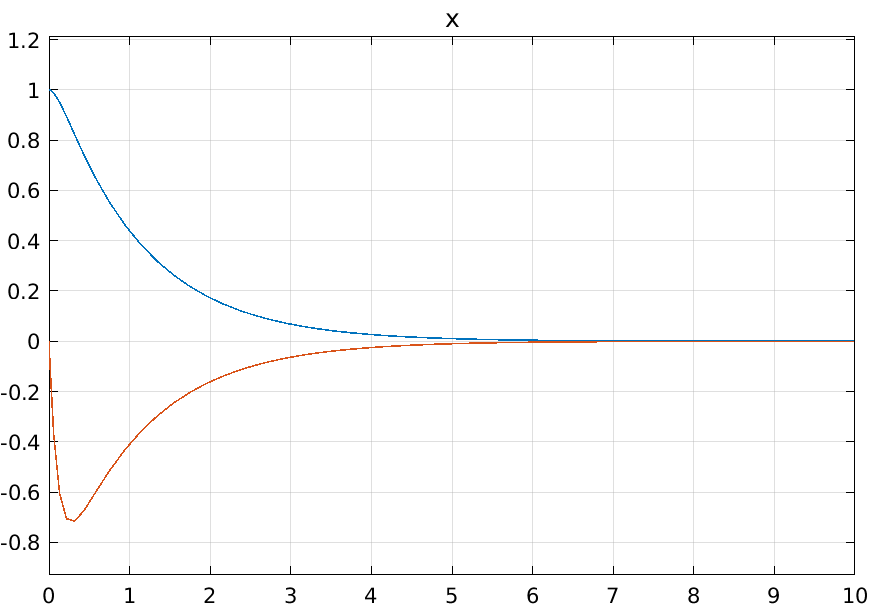
\includegraphics[width=0.59\textwidth]{x-3-plus}
		\caption{Вектор состояния системы $x$ при отклонении $K+1$}
		\label{fig:x-3-plus}
	\end{figure}
	
	\begin{figure}[H]
		\centering
		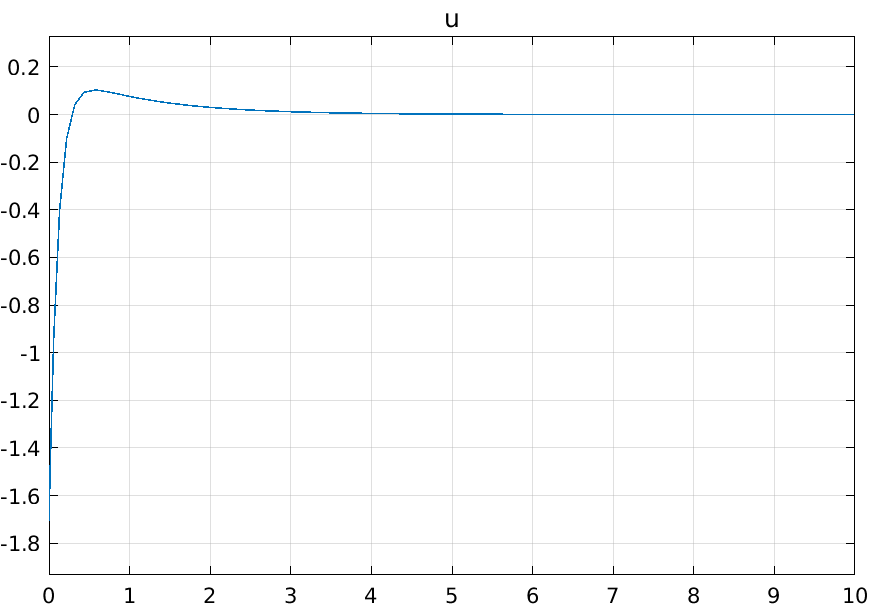
\includegraphics[width=0.59\textwidth]{u-3-plus}
		\caption{Управляющий сигнал $u$ при отклонении $K+1$}
		\label{fig:u-3-plus}
	\end{figure}
	
	\begin{figure}[H]
		\centering
		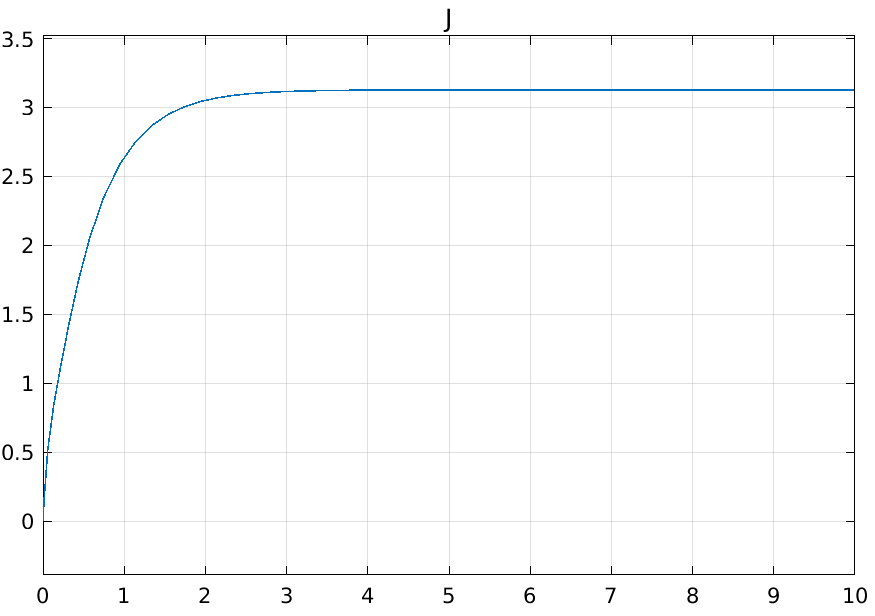
\includegraphics[width=0.59\textwidth]{J-3-plus}
		\caption{Критерий качества $J$ при отклонении $K+1$}
		\label{fig:J-3-plus}
	\end{figure}
	
	Время переходного процесса практически не изменилось, но увеличились предельные значения управляющего сигнала $u$. Также увеличилось установившееся значение критерия качества $J$.
	
	При отрицательном отклонении $K-1$ система расходится, поэтому промоделируем систему при $K-0,5$. Полученные графики представлены на рисунках \ref{fig:x-3-minus}--\ref{fig:J-3-minus}.

	\begin{figure}[H]
		\centering
		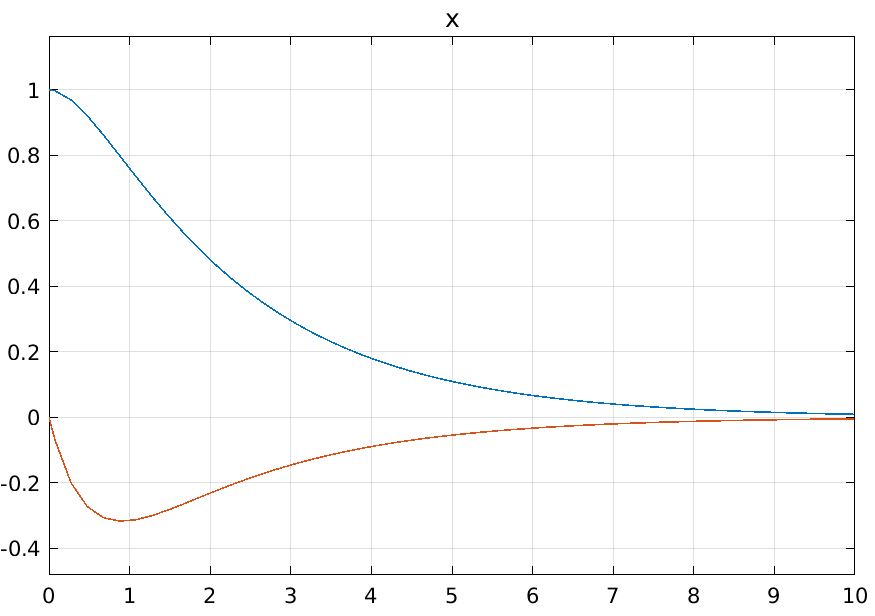
\includegraphics[width=0.59\textwidth]{x-3-minus}
		\caption{Вектор состояния системы $x$ при отклонении $K-0,5$}
		\label{fig:x-3-minus}
	\end{figure}
	
	\begin{figure}[H]
		\centering
		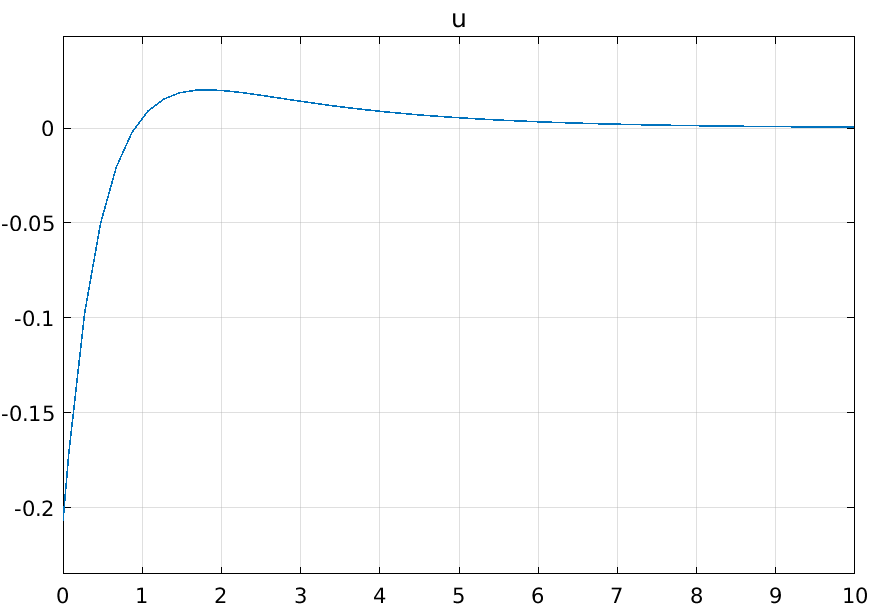
\includegraphics[width=0.59\textwidth]{u-3-minus}
		\caption{Управляющий сигнал $u$ при отклонении $K-0,5$}
		\label{fig:u-3-minus}
	\end{figure}
	
	\begin{figure}[H]
		\centering
		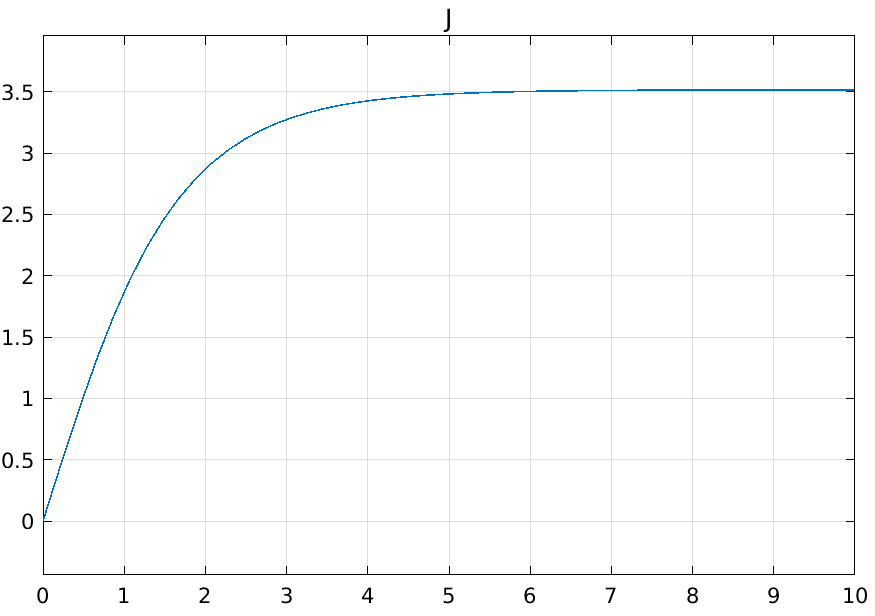
\includegraphics[width=0.59\textwidth]{J-3-minus}
		\caption{Критерий качества $J$ при отклонении $K-0,5$}
		\label{fig:J-3-minus}
	\end{figure}
	
	Время переходного процесса и установившееся значение критерия качества $J$ увеличились.
	
	Проведем моделирование для трех разных значений параметра $r$. Полученные графики при $r=1$, $r=2$, $r=3$ представлены на рисунках \ref{fig:x-4-r1}--\ref{fig:J-4-r3}.
	
	Также проведем моделирование для трех разных матриц $Q$. Полученные графики при $k=0,5$, $k=2$, $k=3$ представлены на рисунках \ref{fig:x-4-k05}--\ref{fig:J-4-k3}.
	
	Можно сделать вывод, что при увеличении как параметра $r$, так и  положительного множителя $k$, увеличиваются предельные значения управляющего сигнала $u$ и установившееся значение критерия качества $J$.
	
	\begin{figure}[H]
		\centering
		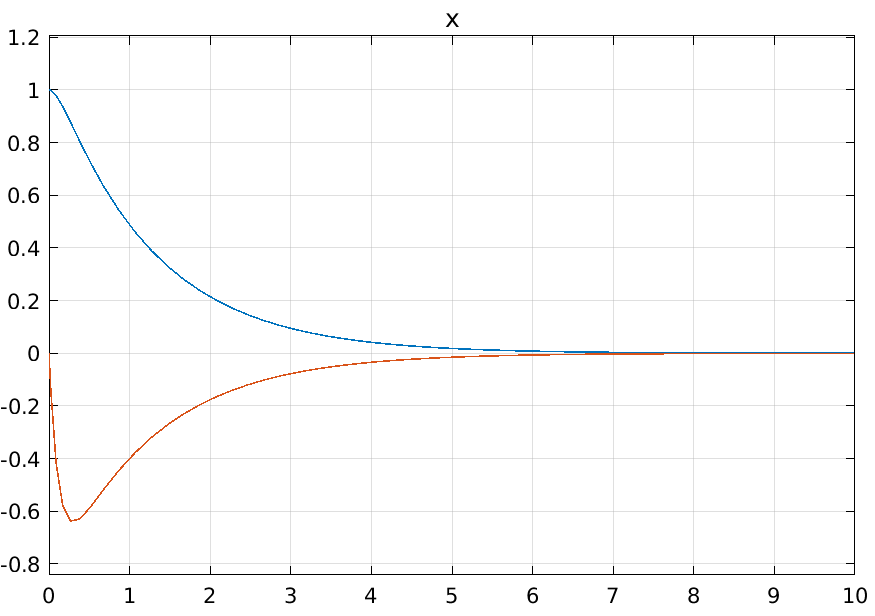
\includegraphics[width=0.59\textwidth]{x-4-r1}
		\caption{Вектор состояния системы $x$ при $r=1$}
		\label{fig:x-4-r1}
	\end{figure}
	
	\begin{figure}[H]
		\centering
		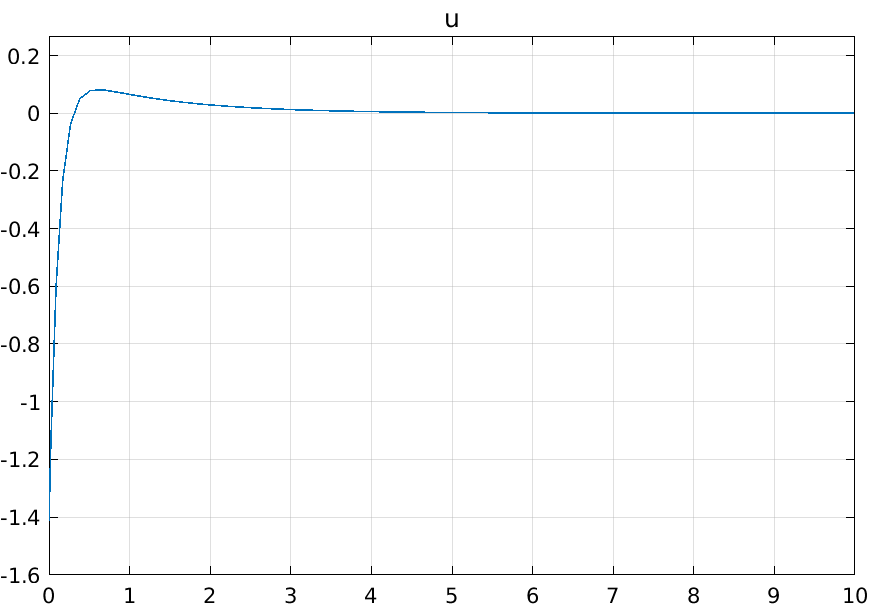
\includegraphics[width=0.59\textwidth]{u-4-r1}
		\caption{Управляющий сигнал $u$ при $r=1$}
		\label{fig:u-4-r1}
	\end{figure}
	
	\begin{figure}[H]
		\centering
		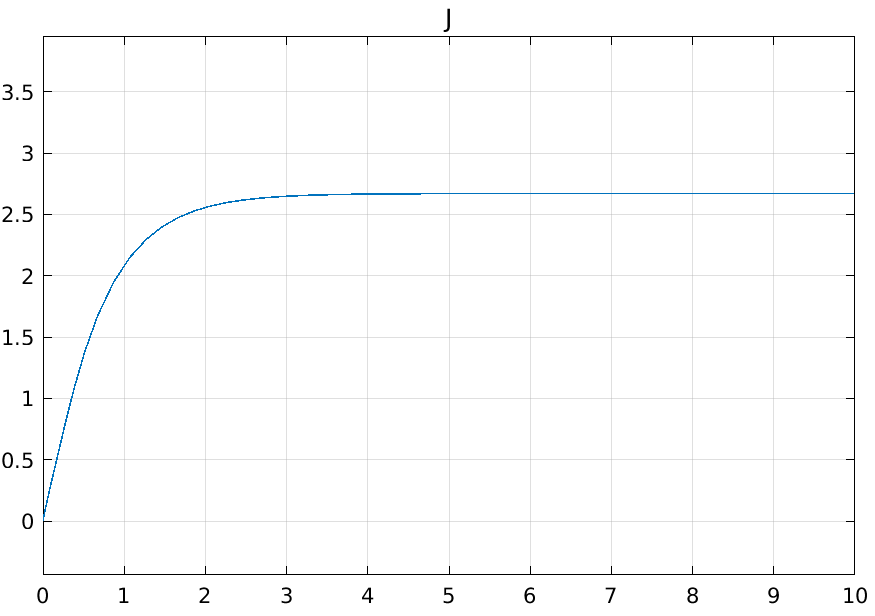
\includegraphics[width=0.59\textwidth]{J-4-r1}
		\caption{Критерий качества $J$ при $r=1$}
		\label{fig:J-4-r1}
	\end{figure}

	\begin{figure}[H]
		\centering
		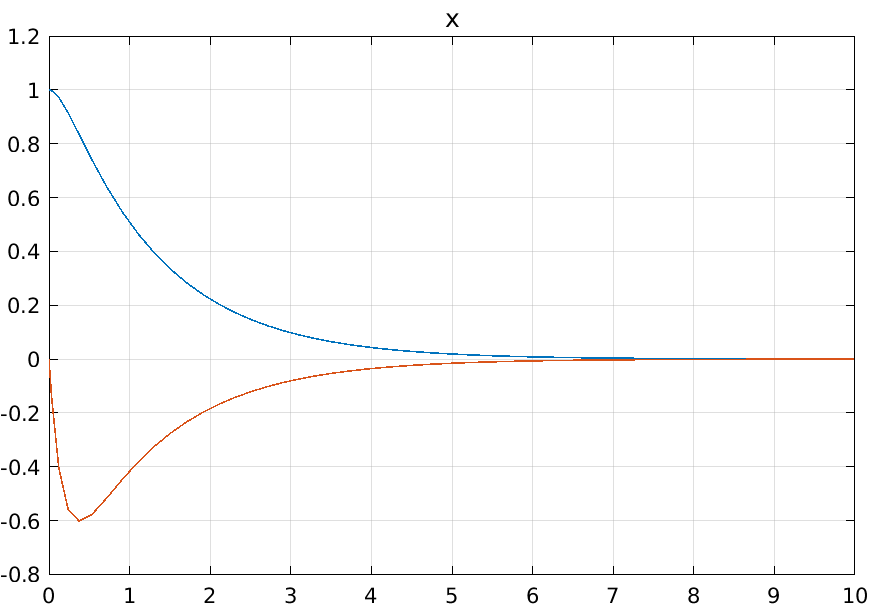
\includegraphics[width=0.59\textwidth]{x-4-r2}
		\caption{Вектор состояния системы $x$ при $r=2$}
		\label{fig:x-4-r2}
	\end{figure}
	
	\begin{figure}[H]
		\centering
		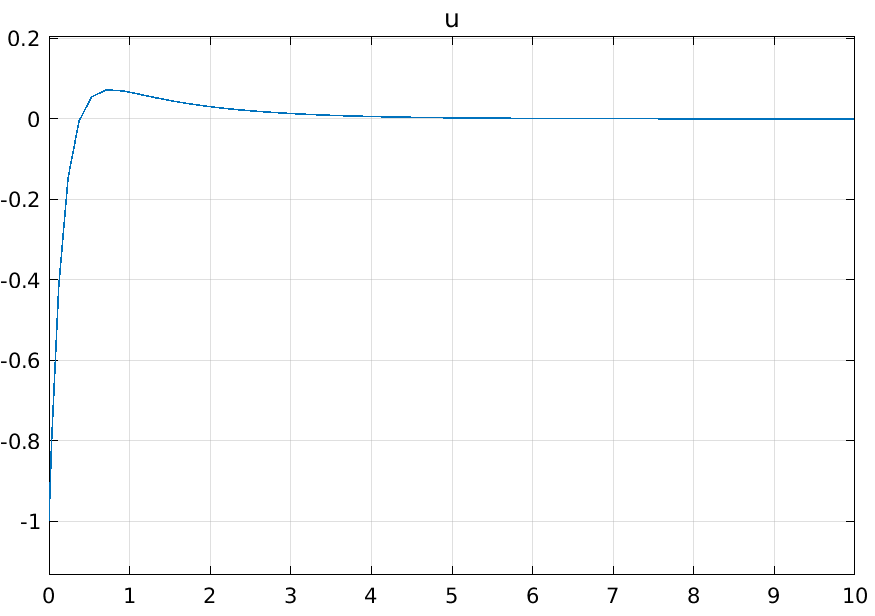
\includegraphics[width=0.59\textwidth]{u-4-r2}
		\caption{Управляющий сигнал $u$ при $r=2$}
		\label{fig:u-4-r2}
	\end{figure}
	
	\begin{figure}[H]
		\centering
		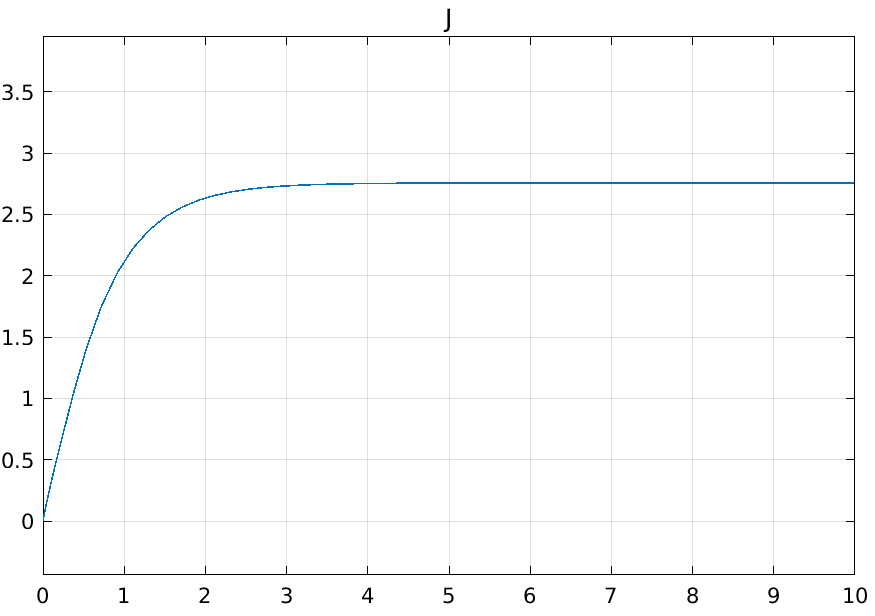
\includegraphics[width=0.59\textwidth]{J-4-r2}
		\caption{Критерий качества $J$ при $r=2$}
		\label{fig:J-4-r2}
	\end{figure}

	\begin{figure}[H]
		\centering
		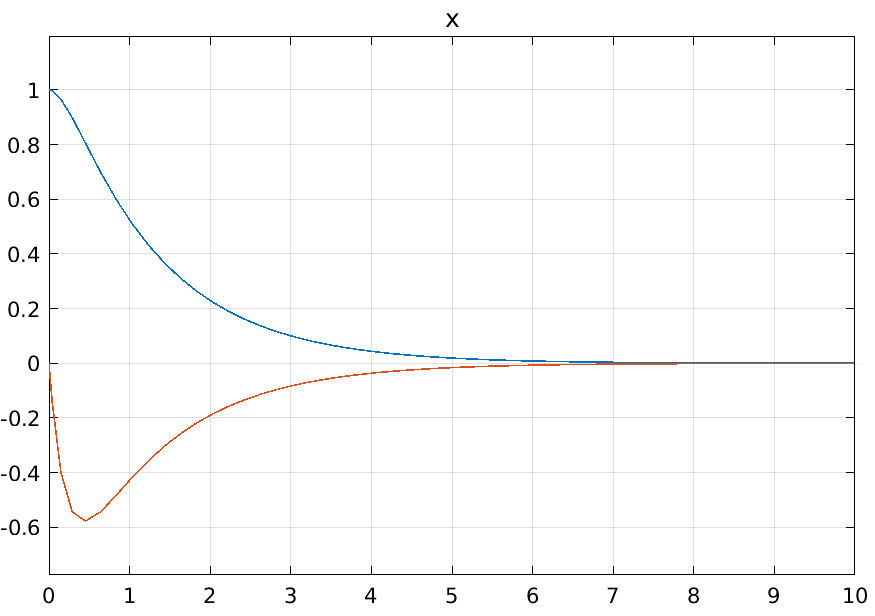
\includegraphics[width=0.59\textwidth]{x-4-r3}
		\caption{Вектор состояния системы $x$ при $r=3$}
		\label{fig:x-4-r3}
	\end{figure}
	
	\begin{figure}[H]
		\centering
		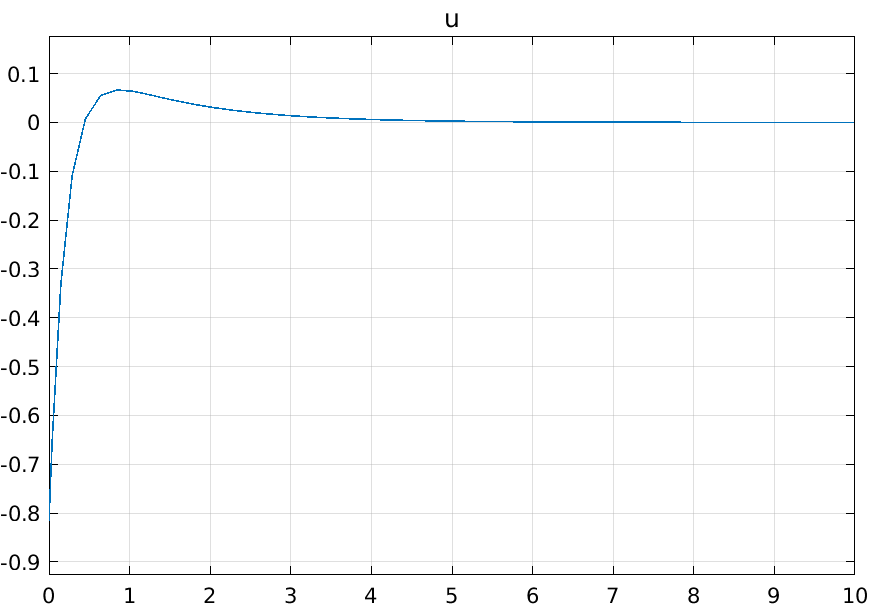
\includegraphics[width=0.59\textwidth]{u-4-r3}
		\caption{Управляющий сигнал $u$ при $r=3$}
		\label{fig:u-4-r3}
	\end{figure}
	
	\begin{figure}[H]
		\centering
		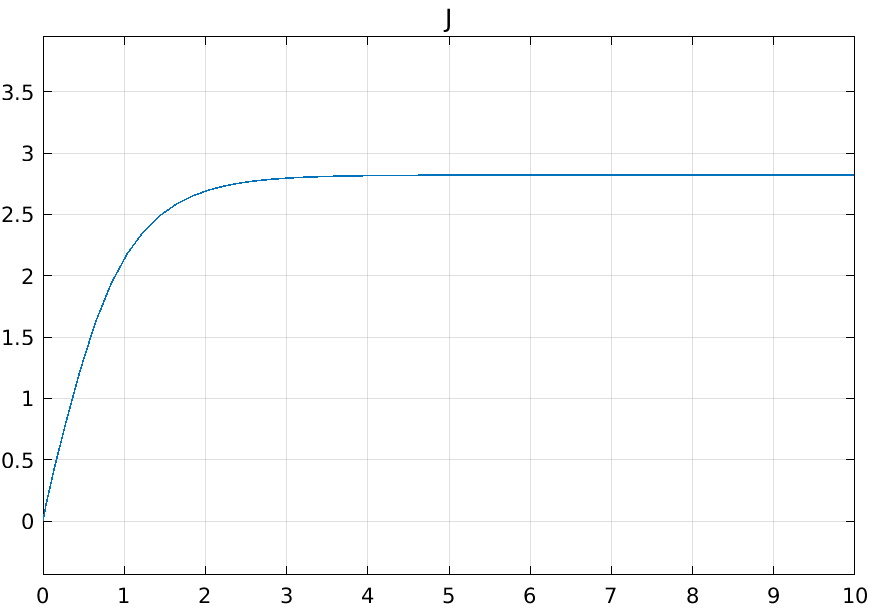
\includegraphics[width=0.59\textwidth]{J-4-r3}
		\caption{Критерий качества $J$ при $r=3$}
		\label{fig:J-4-r3}
	\end{figure}
	
	\begin{figure}[H]
		\centering
		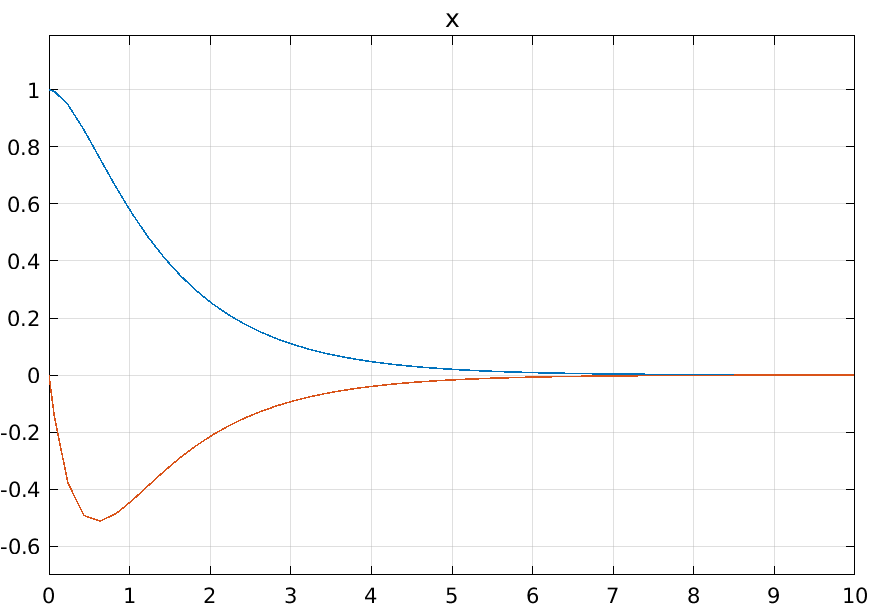
\includegraphics[width=0.59\textwidth]{x-4-k05}
		\caption{Вектор состояния системы $x$ при $k=0,5$}
		\label{fig:x-4-k05}
	\end{figure}
	
	\begin{figure}[H]
		\centering
		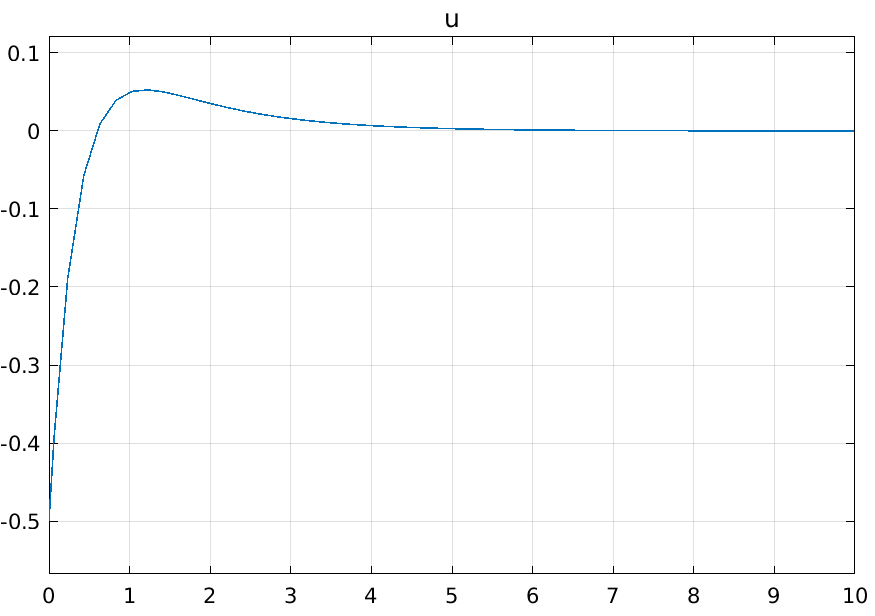
\includegraphics[width=0.59\textwidth]{u-4-k05}
		\caption{Управляющий сигнал $u$ при $k=0,5$}
		\label{fig:u-4-k05}
	\end{figure}
	
	\begin{figure}[H]
		\centering
		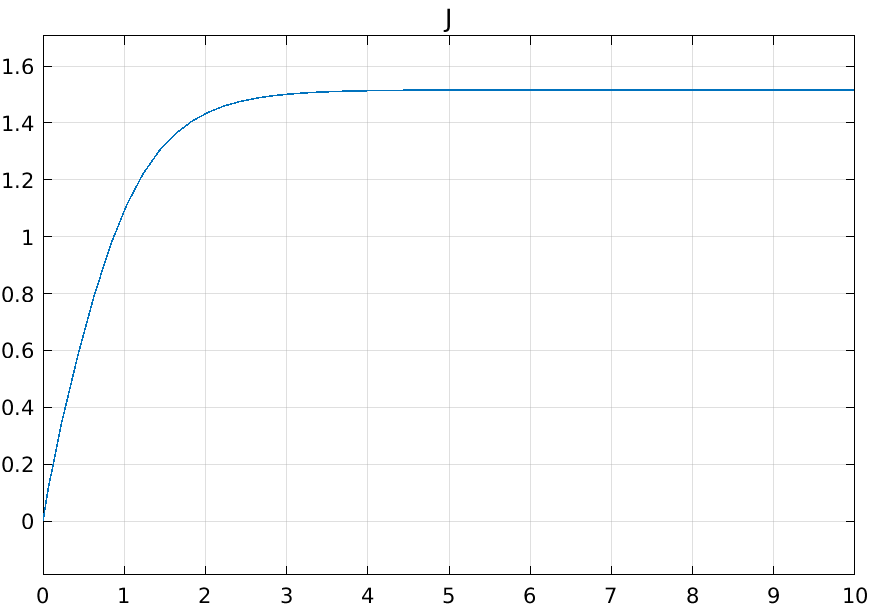
\includegraphics[width=0.59\textwidth]{J-4-k05}
		\caption{Критерий качества $J$ при $k=0,5$}
		\label{fig:J-4-k05}
	\end{figure}

	\begin{figure}[H]
		\centering
		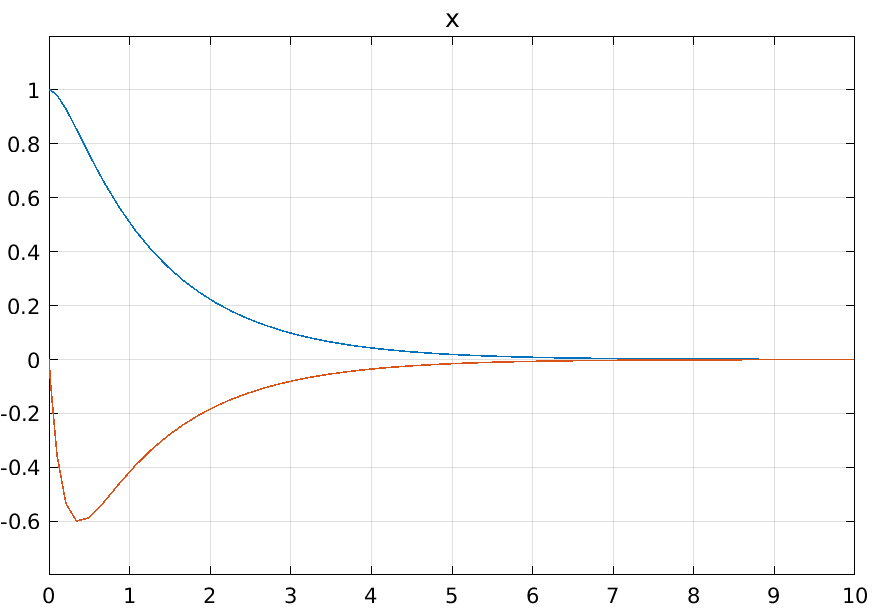
\includegraphics[width=0.59\textwidth]{x-4-k2}
		\caption{Вектор состояния системы $x$ при $k=2$}
		\label{fig:x-4-k2}
	\end{figure}
	
	\begin{figure}[H]
		\centering
		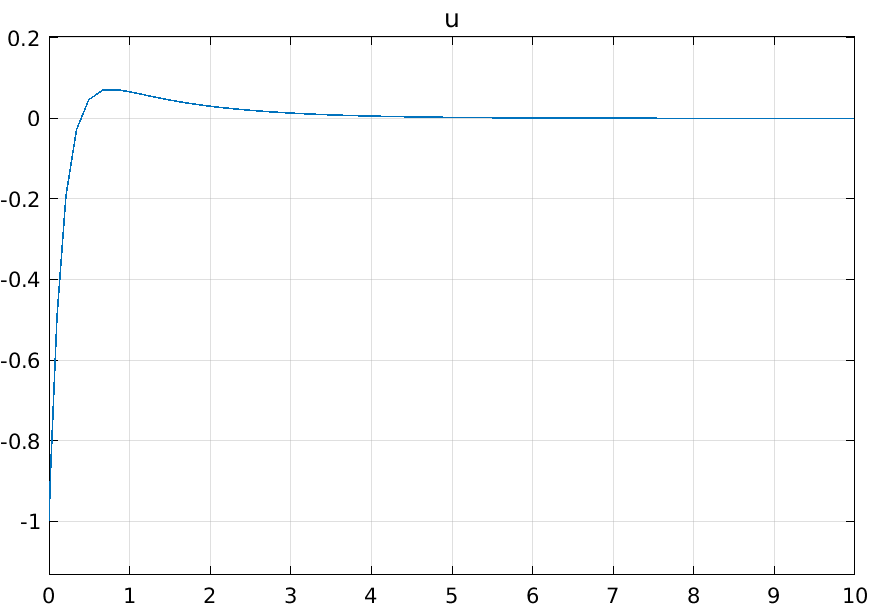
\includegraphics[width=0.59\textwidth]{u-4-k2}
		\caption{Управляющий сигнал $u$ при $k=2$}
		\label{fig:u-4-k2}
	\end{figure}
	
	\begin{figure}[H]
		\centering
		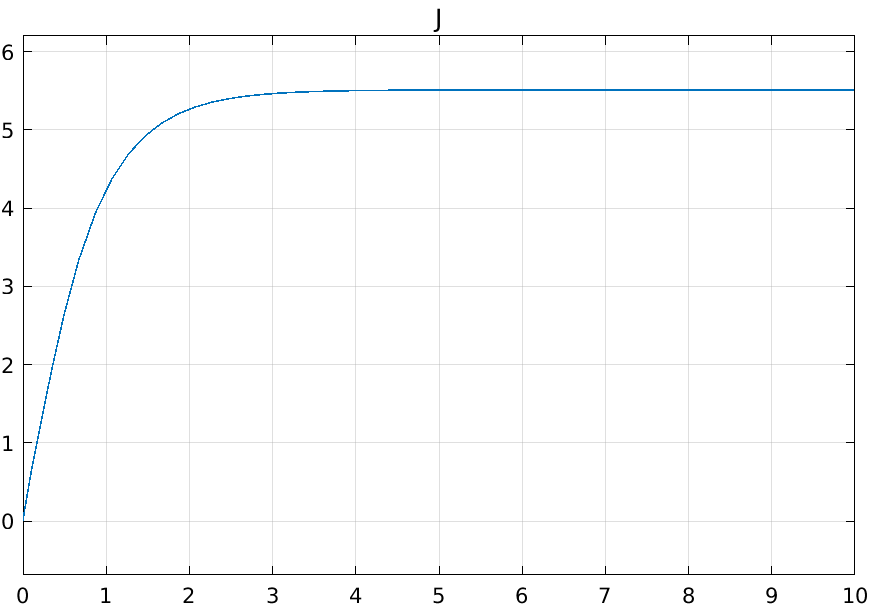
\includegraphics[width=0.59\textwidth]{J-4-k2}
		\caption{Критерий качества $J$ при $k=2$}
		\label{fig:J-4-k2}
	\end{figure}
	
		\begin{figure}[H]
		\centering
		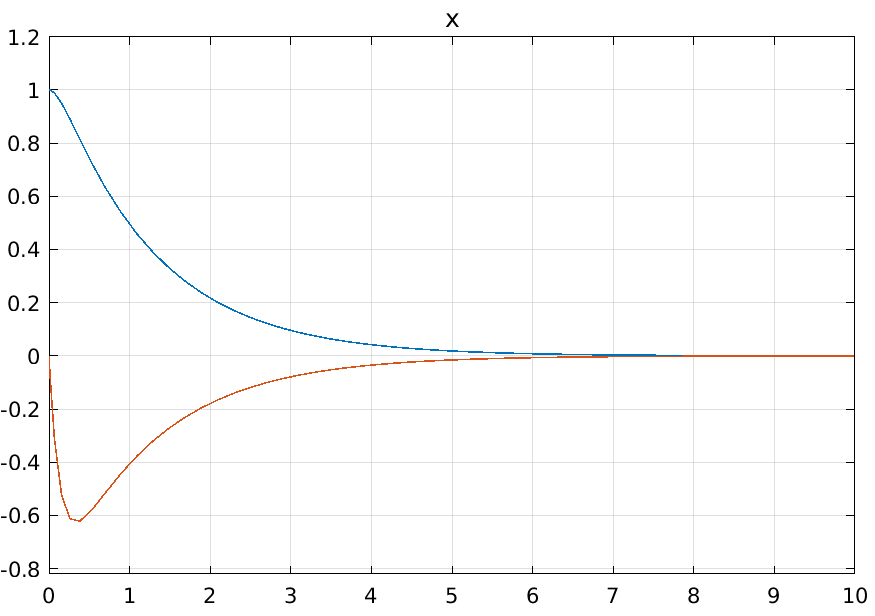
\includegraphics[width=0.59\textwidth]{x-4-k3}
		\caption{Вектор состояния системы $x$ при $k=3$}
		\label{fig:x-4-k3}
	\end{figure}
	
	\begin{figure}[H]
		\centering
		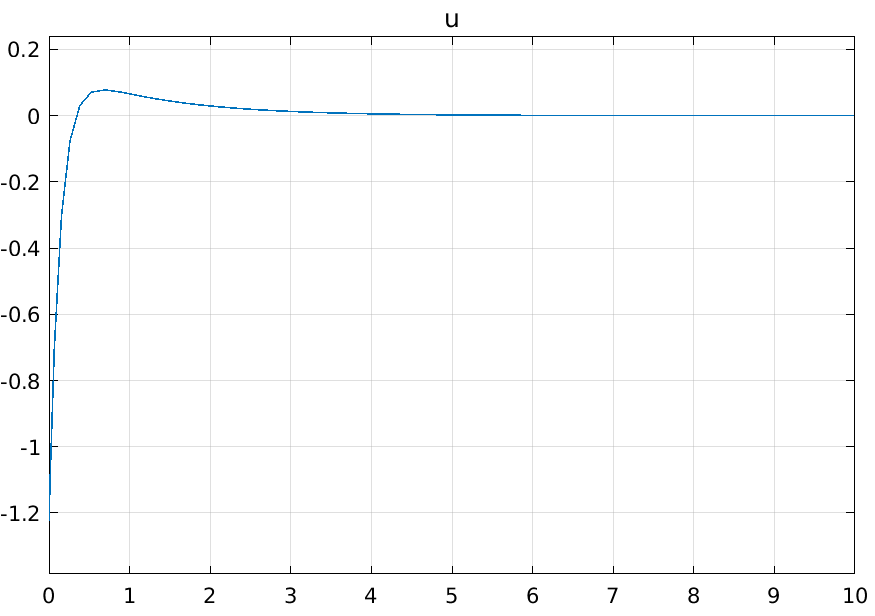
\includegraphics[width=0.59\textwidth]{u-4-k3}
		\caption{Управляющий сигнал $u$ при $k=3$}
		\label{fig:u-4-k3}
	\end{figure}
	
	\begin{figure}[H]
		\centering
		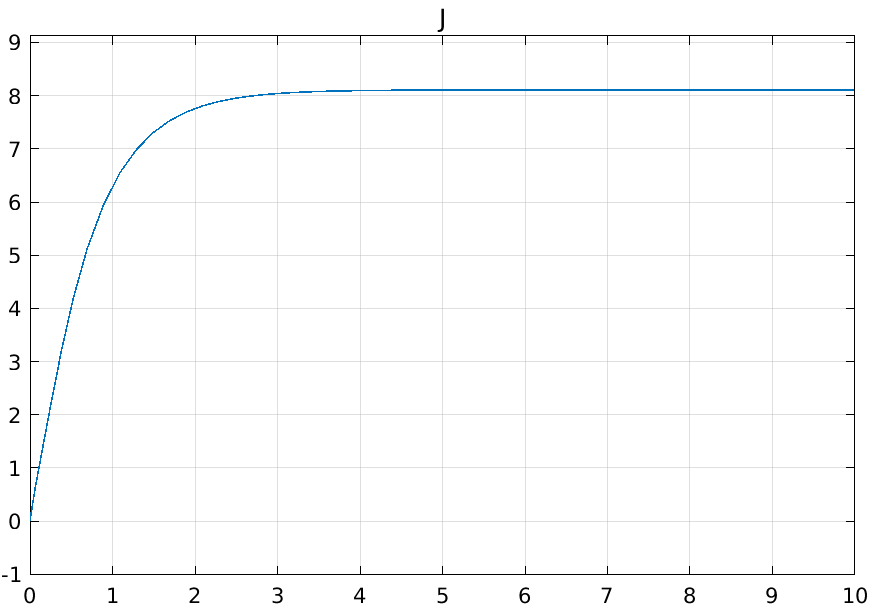
\includegraphics[width=0.59\textwidth]{J-4-k3}
		\caption{Критерий качества $J$ при $k=3$}
		\label{fig:J-4-k3}
	\end{figure}

	\section*{Вывод}
	
	Для системы в соответствии с вариантом задания установившееся значение критерия качества $J=2,8739$.
	
	При отклонении расчетного значения $K$ значение критерия качества растет, что соответствует ухудшению оптимизации управления системы.
	
	Также в работе было доказано, что при увеличении как параметра $r$, так и  положительного множителя $k$, увеличивается установившееся значение критерия качества $J$, что полностью соответствует формулам расчета.
	
\end{document}